\documentclass[../../main.tex]{subfiles}
\graphicspath{{../../image/}{../../figure/}}
\begin{document}

\section{确定性的自编码器}\label{section:ch19-确定性自编码器}

在研究主成分分析（Principal Component Analysis，PCA）时，我们遇到了一种形式简单的自编码器。这种模型通过对输入向量进行线性变换，将其映射到一个低维的流形上，然后通过再次线性变换，将其近似地重构回原始数据空间中（参见\cref{section:ch16-主成分分析}）。我们可以利用神经网络的非线性特点来定义一种非线性 PCA，其中的潜在流形不再是数据空间的线性子空间。这是通过使用输出数量与输入数量相同的网络，并针对每一组训练数据，通过优化权重以最小化输入与输出之间的某种重建误差来实现的。

简单的自编码器在现代深度学习中很少直接使用，因为它们在潜空间中既不能提供语义上有意义的表示，也不能直接从数据分布中生成新的样本。然而，它们为一些更强大的深度生成式模型（如变分自编码器）提供了重要的概念基础（参见\cref{section:ch19-变分自编码器}）。

\subsection{线性自编码器}\label{subsection:ch19-线性自编码器}

首先考虑\cref{figure:ch19-线性自编码器}所示形式的多层感知机，它有 $D$ 个输入单元、$D$ 个输出单元和 $M$ 个隐藏单元，其中 $M<D$。用来训练网络的目标向量就是输入向量本身，因此该网络试图将每个输入向量映射到其自身。由于隐藏单元的数量少于输入单元的数量，它通常无法完美地重构所有输入向量；因此，我们先定义一个误差函数，用来衡量输入向量及其重建之间的不匹配程度，然后通过最小化这个误差函数来确定网络参数 $\bm{w}$。

\begin{definition}[线性自编码器]\label{definition:ch19-线性自编码器}
若\cref{definition:ch19-自编码器}所定义网络的隐藏单元采用线性激活函数，则称它为\textbf{线性自编码器}（linear autoencoder）。它的训练通过最小化如下形式的平方和误差函数来实现：
\begin{align}
E(\bm{w})=\frac{1}{2}\sum_{n=1}^{N}\big\|\bm{y}(\bm{x}_n,\bm{w})-\bm{x}_n\big\|^{2},
\label{align:ch19-平方和误差}
\end{align}
其中 $\bm{y}(\bm{x}_n,\bm{w})$ 是网络对输入 $\bm{x}_n$ 的重建。
\end{definition}

% SUPPLEMENT: parent=definition:ch19-线性自编码器; kind=motivation; location=紧随其后的 remark（重构新增）
\begin{remark}（重构新增）
\cref{definition:ch19-线性自编码器}中的式\eqref{align:ch19-平方和误差}取 $\frac{1}{2}$ 的因子并不是数学上的需要，而是为了让求导后消去平方项的系数 $2$，使梯度形式更干净；把它换成任意正常数只会整体缩放误差曲面，不改变极小点。这里把“线性”加在\emph{隐藏单元}上而不是加在输出单元上，是因为输出单元本来就是线性的（否则 $\bm{y}(\bm{x}_n,\bm{w})$ 无法与 $\bm{x}_n$ 直接比较）：真正决定模型容量的是隐藏层。条件 $M<D$ 是这一节的核心约束，它使 $\bm{B}\bm{A}$ 的秩不超过 $M$，从而排除了 $\bm{B}\bm{A}=\bm{I}$ 这种把输入原样复制的平凡解；若去掉它，取 $\bm{A}=\bm{I}$、$\bm{B}=\bm{I}$ 就有 $E(\bm{w})=0$，训练失去意义。注意误差中并没有显式地减去数据均值，这一点在\cref{theorem:ch19-线性AE与PCA}之后的注记中还会讨论。
\end{remark}

\begin{figure}[htbp]
\centering
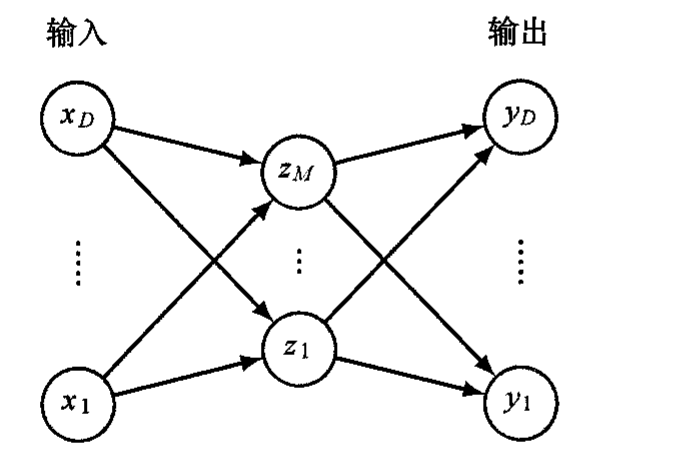
\includegraphics[width=0.58\textwidth]{ch19-fig510-linear-ae.png}
\caption{一个具有两层权重的多层感知机。这样的网络是通过最小化平方和误差来训练的，使得输入向量被映射到它们自身。即使隐藏层中有非线性单元，这样的网络也相当于线性主成分分析。为了清晰起见，表示偏置参数的连接已省略}
\label{figure:ch19-线性自编码器}
\end{figure}

\begin{theorem}[线性自编码器的最优解与主成分分析]\label{theorem:ch19-线性AE与PCA}
设训练数据 $\bm{x}_1,\cdots,\bm{x}_N\in\mathbb{R}^{D}$，记 $\bm{S}=\sum_{n=1}^{N}\bm{x}_n\bm{x}_n^{\mathsf T}$。设 $\bm{S}$ 的特征值为 $\lambda_1\geqslant\lambda_2\geqslant\cdots\geqslant\lambda_D\geqslant0$，对应的单位正交特征向量为 $\bm{u}_1,\cdots,\bm{u}_D$。设线性自编码器的隐藏层宽为 $M<D$，隐藏层与输出层都是线性的，即存在 $\bm{A}\in\mathbb{R}^{M\times D}$ 与 $\bm{B}\in\mathbb{R}^{D\times M}$，使得
\begin{align*}
\bm{z}(\bm{x})=\bm{A}\bm{x},\qquad \bm{y}(\bm{x})=\bm{B}\bm{A}\bm{x}.
\end{align*}
则：
\begin{enumerate}[(i)]
\item 误差函数\eqref{align:ch19-平方和误差}的全局最小值唯一，且等于 $\frac{1}{2}\sum_{i=M+1}^{D}\lambda_i$；
\item 当 $\lambda_M>\lambda_{M+1}$ 且 $\bm{S}$ 正定时，该最小值当且仅当 $\bm{B}\bm{A}$ 是到 $\operatorname{span}\{\bm{u}_1,\cdots,\bm{u}_M\}$ 的正交投影时取到；
\item 此时网络执行一个投影操作，把数据映射到由数据的前 $M$ 个主成分所张成的 $M$ 维子空间上，通向隐藏单元的权重向量（即 $\bm{A}$ 的各行）构成该主子空间的一组基；这些向量不必是正交或归一化的。
\end{enumerate}
\end{theorem}
\begin{proof}（重构新增）
记 $\bm{P}=\bm{B}\bm{A}$，则 $\operatorname{rank}\bm{P}\leqslant M$，且
\begin{align*}
E(\bm{w})=\frac{1}{2}\sum_{n=1}^{N}\big\|\bm{x}_n-\bm{P}\bm{x}_n\big\|^{2}.
\end{align*}
分四步证明。

（1）任意 $\bm{P}$ 都可替换为其值域上的正交投影。设 $\bm{Q}$ 是到 $\operatorname{range}(\bm{P})$ 的正交投影，则 $\bm{Q}\bm{P}=\bm{P}$，从而 $(\bm{I}-\bm{Q})\bm{x}_n$ 与 $\operatorname{range}(\bm{P})$ 正交，而 $(\bm{Q}-\bm{P})\bm{x}_n=\bm{Q}\bm{x}_n-\bm{P}\bm{x}_n$ 落在 $\operatorname{range}(\bm{P})$ 中。于是二者正交，由勾股定理，
\begin{align*}
\big\|\bm{x}_n-\bm{P}\bm{x}_n\big\|^{2}=\big\|\bm{x}_n-\bm{Q}\bm{x}_n\big\|^{2}+\big\|\bm{Q}\bm{x}_n-\bm{P}\bm{x}_n\big\|^{2}\geqslant\big\|\bm{x}_n-\bm{Q}\bm{x}_n\big\|^{2}.
\end{align*}
因此只需在秩不超过 $M$ 的正交投影中极小化 $E$，而且（1）中的等号成立当且仅当 $\bm{Q}\bm{x}_n=\bm{P}\bm{x}_n$ 对每个 $n$ 成立。

（2）对秩为 $r\leqslant M$ 的正交投影 $\bm{Q}$，设 $\bm{V}=[\bm{v}_1,\cdots,\bm{v}_r]$ 是 $\operatorname{range}(\bm{Q})$ 的标准正交基，则 $\bm{Q}=\bm{V}\bm{V}^{\mathsf T}$。由 $\bm{Q}$ 的对称性与幂等性，
\begin{align*}
\sum_{n=1}^{N}\big\|\bm{x}_n-\bm{Q}\bm{x}_n\big\|^{2}=\sum_{n=1}^{N}\|\bm{x}_n\|^{2}-\sum_{n=1}^{N}\|\bm{Q}\bm{x}_n\|^{2}=\operatorname{tr}\bm{S}-\operatorname{tr}\big(\bm{V}^{\mathsf T}\bm{S}\bm{V}\big).
\end{align*}
由谱分解（见\hyperref[chapter:appA-线性代数]{附录\ref*{chapter:appA-线性代数}}），$\bm{S}=\bm{U}\bm{\Lambda}\bm{U}^{\mathsf T}$，其中 $\bm{U}=[\bm{u}_1,\cdots,\bm{u}_D]$ 正交、$\bm{\Lambda}=\operatorname{diag}(\lambda_1,\cdots,\lambda_D)$。记 $\bm{C}=\bm{U}^{\mathsf T}\bm{V}$，则 $\bm{C}^{\mathsf T}\bm{C}=\bm{I}_r$，故 $c_i\triangleq\|\bm{C}_{i\cdot}\|^{2}$ 满足 $0\leqslant c_i\leqslant1$ 且 $\sum_{i=1}^{D}c_i=\|\bm{C}\|_F^{2}=r$，并且
\begin{align*}
\operatorname{tr}\big(\bm{V}^{\mathsf T}\bm{S}\bm{V}\big)=\operatorname{tr}\big(\bm{C}^{\mathsf T}\bm{\Lambda}\bm{C}\big)=\sum_{i=1}^{D}\lambda_i c_i\leqslant\sum_{i=1}^{r}\lambda_i,
\end{align*}
最后一个不等号是因为把总量为 $r$ 的权重 $c_i\in[0,1]$ 分配给 $\lambda_i$ 时，最大值出现在把权重全部分配给最大的 $r$ 个 $\lambda_i$ 处；当 $\lambda_r>\lambda_{r+1}$ 时等号成立当且仅当 $c_1=\cdots=c_r=1$、$c_{r+1}=\cdots=c_D=0$，即 $\operatorname{range}(\bm{Q})=\operatorname{span}\{\bm{u}_1,\cdots,\bm{u}_r\}$。于是
\begin{align*}
E\geqslant\frac{1}{2}\Big(\operatorname{tr}\bm{S}-\sum_{i=1}^{r}\lambda_i\Big)=\frac{1}{2}\sum_{i=r+1}^{D}\lambda_i\geqslant\frac{1}{2}\sum_{i=M+1}^{D}\lambda_i.
\end{align*}

（3）取 $\bm{A}=[\bm{u}_1,\cdots,\bm{u}_M]^{\mathsf T}$、$\bm{B}=[\bm{u}_1,\cdots,\bm{u}_M]$，则 $\bm{B}\bm{A}=\sum_{i=1}^{M}\bm{u}_i\bm{u}_i^{\mathsf T}$ 正是到主子空间 $\operatorname{span}\{\bm{u}_1,\cdots,\bm{u}_M\}$ 的正交投影，此时 $E=\frac{1}{2}\sum_{i=M+1}^{D}\lambda_i$，下界可以取到，故最小值等于 $\frac{1}{2}\sum_{i=M+1}^{D}\lambda_i$，它由 $\lambda_{M+1},\cdots,\lambda_D$ 唯一确定。

（4）等号情形的刻画。由（1）（2），当 $\bm{S}$ 正定且 $\lambda_M>\lambda_{M+1}$ 时，$E$ 取到最小值必须有 $r=M$、$\operatorname{range}(\bm{Q})=\operatorname{span}\{\bm{u}_1,\cdots,\bm{u}_M\}$ 且 $\bm{P}\bm{x}_n=\bm{Q}\bm{x}_n$ 对一切 $n$ 成立；$\bm{S}$ 正定意味着 $\{\bm{x}_n\}$ 张成 $\mathbb{R}^{D}$，故 $\bm{P}=\bm{Q}$。此时 $\operatorname{range}(\bm{A}^{\mathsf T})=\operatorname{range}(\bm{P})=\operatorname{span}\{\bm{u}_1,\cdots,\bm{u}_M\}$，所以 $\bm{A}$ 的各行线性无关并构成主子空间的一组基；而 $\bm{A}$ 只受“行空间等于主子空间”这一条件约束，各行一般既不正交也未归一化。最后，使 $E$ 取到最小值的参数 $(\bm{A},\bm{B})$ 并不唯一：对任意可逆的 $\bm{R}\in\mathbb{R}^{M\times M}$，把 $\bm{A}$ 换成 $\bm{R}\bm{A}$、$\bm{B}$ 换成 $\bm{B}\bm{R}^{-1}$ 时 $\bm{B}\bm{A}$ 不变，故误差不变。
\end{proof}

% SUPPLEMENT: parent=theorem:ch19-线性AE与PCA; kind=motivation; location=紧随其后的 remark（重构新增）
\begin{remark}（重构新增）
\cref{theorem:ch19-线性AE与PCA}解释了为什么“线性自编码器不提供超出 PCA 的东西”：两者的目标函数是同一个平方和误差，而 PCA 的主成分正是该误差在秩约束下的最优解，所以训练一个线性自编码器等价于用迭代法计算主成分，结论与 Bourlard and Kamp（1988）、Baldi and Hornik（1989）一致。

逐项说明条件的作用与边界：
\begin{enumerate}[(1)]
\item $M<D$ 与“秩不超过 $M$”是结论的全部内容所在。若 $M\geqslant D$，结论中的下界 $\frac{1}{2}\sum_{i=M+1}^{D}\lambda_i$ 成为空和 $0$，而 $\bm{B}\bm{A}=\bm{I}$ 确实使 $E=0$，此时自编码器退化为恒等映射，与“复制输入不解决任何实际问题”的说法相符。
\item “隐藏层与输出层都是线性的”是证明中把网络写成 $\bm{B}\bm{A}\bm{x}$ 的前提。若隐藏单元取非线性激活函数，上述证明不再适用；但 Bourlard and Kamp（1988）证明了即使隐藏单元非线性，最小误差解仍会被投影到主成分子空间——这是引用结果，本书未给证明，故本定理不覆盖该情形。
\item “平方和误差”使 $E$ 成为 $\bm{P}$ 的二次函数，才能用谱分解把它化为 $\operatorname{tr}\bm{S}-\operatorname{tr}(\bm{V}^{\mathsf T}\bm{S}\bm{V})$。若换成交叉熵等其它损失，最优子空间一般不再是主子空间；原书在\cref{subsection:ch19-深度自编码器}中正是通过加入非线性层而不是更换损失来突破线性限制。
\item 关于数据中心化：\eqref{align:ch19-平方和误差}没有减去均值，证明中的 $\bm{S}$ 是二阶矩矩阵。\cref{figure:ch19-线性自编码器}为清晰起见省略了偏置连接，而偏置的作用恰好等价于先减去均值再重构，因此含偏置的网络对应的是协方差矩阵的谱分解。两种写法只在“是否把均值方向计入子空间”上有差别，不影响 $M<D$ 时的秩约束论证。
\item 关于唯一性：最小\emph{值}唯一（它只依赖 $\lambda_{M+1},\cdots,\lambda_D$），但取到最小值的\emph{参数}不唯一（见证明（4））；当 $\lambda_M=\lambda_{M+1}$ 时主子空间本身也不唯一，此时结论（3）中的“该主子空间”应理解为任一由前 $M$ 个特征向量张成的子空间。
\item 关于 $\bm{S}$ 不满秩：若 $N<D$ 或数据退化，$\bm{S}$ 只有 $r_0<D$ 个正特征值。此时下界仍为 $\frac{1}{2}\sum_{i=M+1}^{D}\lambda_i$（其中 $\lambda_i=0$ 的项不贡献），但等号条件只在 $\operatorname{span}\{\bm{x}_1,\cdots,\bm{x}_N\}$ 上成立，这正是\cref{theorem:ch19-线性AE与PCA}中附加“$\bm{S}$ 正定”的原因。
\end{enumerate}
\end{remark}

这个结果并不在意料之外，因为 PCA 和神经网络都依赖于线性降维以及最小化相同的平方和误差函数。

有人可能会觉得，对\cref{figure:ch19-线性自编码器}所示网络的隐藏单元使用非线性激活函数，可以克服线性流形的局限性。然而，即使有非线性隐藏单元，最小误差解也仍然会被投影到主成分子空间（Bourlard and Kamp，1988）。因此，使用两层神经网络进行降维没有任何优势。基于奇异值分解（SVD）的标准 PCA 技术可以保证在有限时间内给出正确解，并且生成一组有序的特征值及对应的正交归一化特征向量。

\subsection{深度自编码器}\label{subsection:ch19-深度自编码器}

然而，如果在网络中加入额外的非线性层，情况就有所不同了。

\begin{definition}[深度自编码器]\label{definition:ch19-深度自编码器}
称\cref{figure:ch19-深度自编码器}所示形式的四层自联想网络为\textbf{深度自编码器}（deep autoencoder）：它的输出单元仍然是线性的，第二层中的 $M$ 个单元也可以是线性的，而第一层和第三层具有非线性激活函数；它仍然通过最小化损失函数\eqref{align:ch19-平方和误差}来训练。
\end{definition}

% SUPPLEMENT: parent=definition:ch19-深度自编码器; kind=motivation; location=紧随其后的 remark（重构新增）
\begin{remark}（重构新增）
\cref{definition:ch19-深度自编码器}中“两层非线性夹一层线性”的结构不是随意的：若第一层也是线性的，则整个网络仍是 $\bm{B}\bm{A}\bm{x}$ 的形式，\cref{theorem:ch19-线性AE与PCA}立即适用，非线性层就白加了；若第二层也非线性，则中间的 $M$ 个单元只是又一层非线性特征，“$M$ 维子空间的坐标”这一几何解释便不再适用，但网络作为非线性降维器仍然成立。因此“第一层、第三层非线性、第二层线性”恰好保证了 $F_1$ 可以是任意非线性映射而 $F_2$ 在其参数化下仍把 $M$ 维潜空间嵌入 $\mathbb{R}^{D}$。

条件的代价在于优化：\eqref{align:ch19-平方和误差}不再是 $\bm{w}$ 的二次函数，全局最小值一般无法用闭式解或凸优化得到，只能依赖局部搜索，因而存在收敛到次优局部极小值的风险；此外潜空间维数 $M$ 必须在训练之前人为指定，不能像概率 PCA 那样由数据自动确定（参见\cref{section:ch16-概率潜变量}）。
\end{remark}

我们可以将这个网络视为两个连续的函数映射（下文简称映射）$F_1$ 和 $F_2$，如\cref{figure:ch19-深度自编码器}所示。第一个映射 $F_1$ 将原始的 $D$ 维数据投影到了由第二层单元的激活定义的 $M$ 维子空间。因为第一层非线性单元的存在，这个映射非常通用，不受限于线性映射。类似地，该网络的后半部分定义了从 $M$ 维隐藏空间回到原始 $D$ 维输入空间的任意映射。这在几何上有一个简单的解释，参见\cref{figure:ch19-流形嵌入}，其中 $D=3$ 且 $M=2$。

\begin{figure}[htbp]
\centering
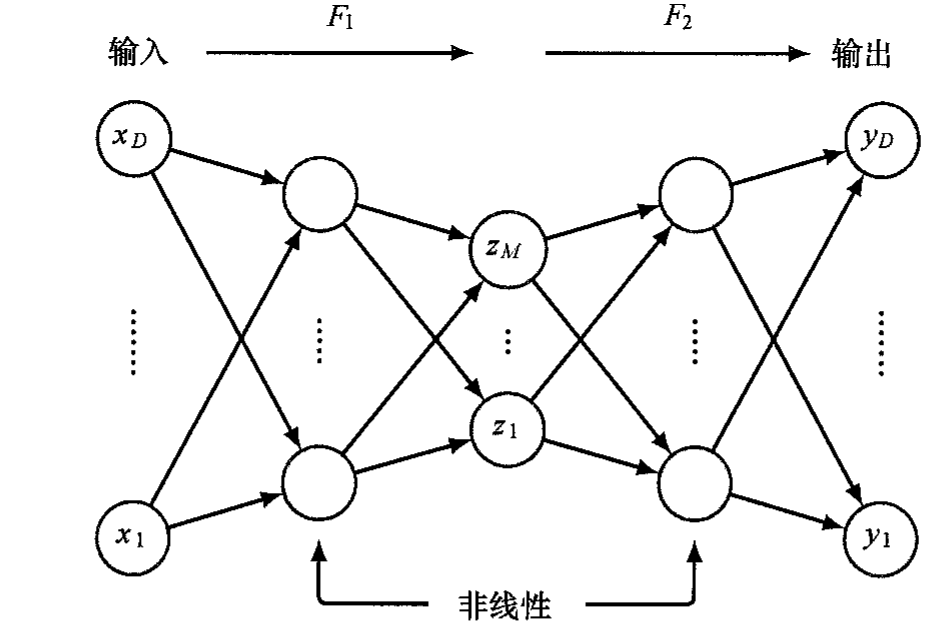
\includegraphics[width=0.72\textwidth]{ch19-fig511-deep-ae.png}
\caption{添加额外的非线性单元隐藏层会产生一个自联想网络，它可以执行非线性降维}
\label{figure:ch19-深度自编码器}
\end{figure}

\begin{figure}[htbp]
\centering
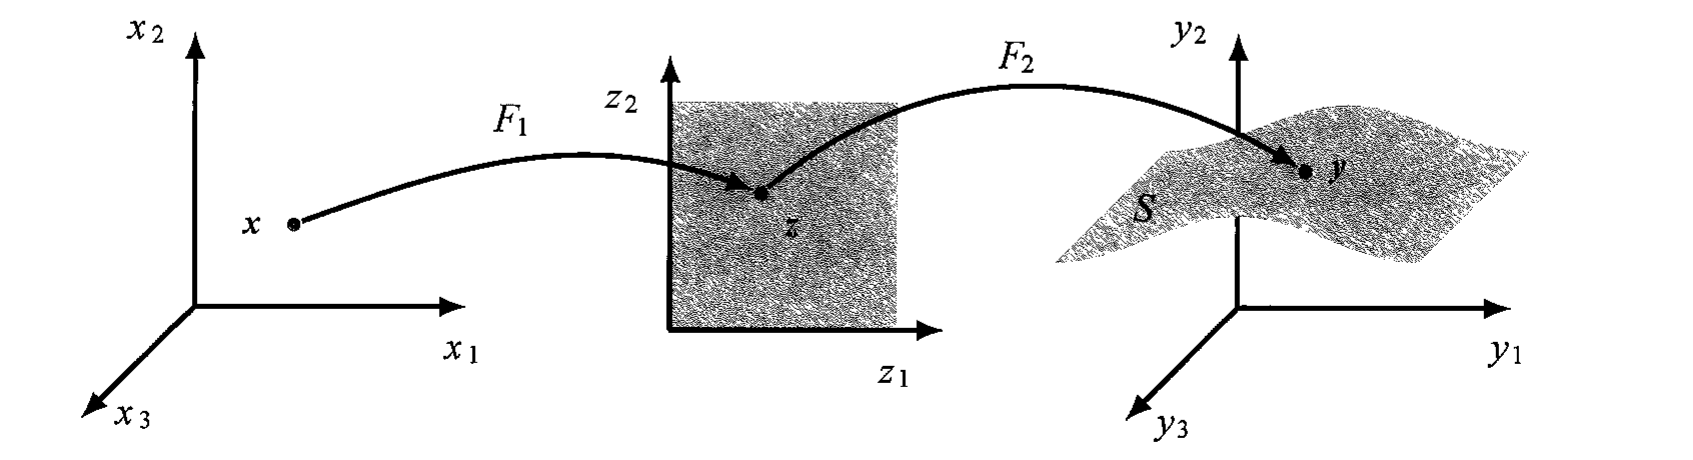
\includegraphics[width=0.95\textwidth]{ch19-fig511-manifold.png}
\caption{\cref{figure:ch19-深度自编码器}所示网络执行的映射的几何解释（具有 $D=3$ 个输入且第二层中有 $M=2$ 个单元的模型）从潜空间到数据空间的映射 $F_2$ 定义了流形 $S$ 在更高维数据空间中的嵌入方式。由于映射 $F_2$ 可以是非线性的，因此流形 $S$ 的嵌入可以是非平面的。映射 $F_1$ 则定义了从原始 $D$ 维数据空间到 $M$ 维潜空间的投影}
\label{figure:ch19-流形嵌入}
\end{figure}

这样的网络实际上有效地执行了一种非线性形式的 PCA。它具有不受限于线性变换的优势，尽管标准 PCA 是它的一个特例。然而，现在训练网络需要进行非线性优化，因为误差函数\eqref{align:ch19-平方和误差}不再是网络参数的二次函数。因此必须使用计算密集型的非线性优化技术，并且存在找到误差函数的次优局部极小值的风险。此外，在训练网络之前必须指定子空间的维数。

\subsection{稀疏自编码器}\label{subsection:ch19-稀疏自编码器}

与其限制网络中某个隐藏层的节点数量，不如考虑另一种约束内部表示的方法：使用正则化器鼓励稀疏表示，从而降低有效维度。一个简单的选择是 $L_1$ 正则化器，它能促进数据的稀疏性，相应的正则化误差函数如下（参见\cref{subsection:ch09-广义权重衰减}）：

\begin{definition}[稀疏自编码器]\label{definition:ch19-稀疏自编码器}
在自编码器的误差函数中加入对隐藏单元激活值的 $L_1$ 惩罚，得到\textbf{正则化误差函数}
\begin{align}
\tilde{E}(\bm{w})=E(\bm{w})+\lambda\sum_{k=1}^{K}|z_k|,
\label{align:ch19-稀疏正则}
\end{align}
其中 $z_k$ 是隐藏层中第 $k$ 个单元的激活值，$K$ 是隐藏层单元数，$\lambda>0$ 是正则化系数。用\eqref{align:ch19-稀疏正则}训练的自编码器称为\textbf{稀疏自编码器}（sparse autoencoder）。
\end{definition}

% SUPPLEMENT: parent=definition:ch19-稀疏自编码器; kind=motivation; location=紧随其后的 remark（重构新增）
\begin{remark}（重构新增）
\cref{definition:ch19-稀疏自编码器}最容易被忽略的一点是：正则化施加在\emph{单元激活值} $z_k$ 上，而不是像通常的权重衰减那样施加在网络参数 $\bm{w}$ 上（参见\cref{subsection:ch09-广义权重衰减}）。两者作用的对象不同，效果也不同：对 $\bm{w}$ 的 $L_1$ 惩罚压缩的是权重，而对 $z_k$ 的 $L_1$ 惩罚直接推动隐藏层在给定输入下只有少数单元被激活，从而“降低有效维度”而不必真的删掉单元。这也是它被称为“另一种约束内部表示的方法”的原因——它不是通过减少单元数 $M$ 来限制容量，而是在 $M$ 不变的前提下让表示变稀疏。

$\lambda$ 控制稀疏性与重建精度之间的取舍：$\lambda$ 太小则\eqref{align:ch19-稀疏正则}退化为原来的平方和误差，稀疏性无从产生；$\lambda$ 太大则网络倾向于令所有 $z_k$ 都接近于零，重建误差随之上升。注意 $|z_k|$ 在 $z_k=0$ 处不可微，实践中要么使用自动微分框架的次梯度约定，要么把 $|z_k|$ 换成光滑近似（如 $\sqrt{z_k^{2}+\varepsilon}$）；原书只说明“导数可以像往常一样使用自动微分来计算”，并未讨论这一细节。最后，\eqref{align:ch19-稀疏正则}对 $z_k$ 的依赖使得误差不再只是 $\bm{w}$ 的二次函数，即使在“线性”自编码器中也不能再用\cref{theorem:ch19-线性AE与PCA}的谱分解方法求闭式解。
\end{remark}

其中 $E(\bm{w})$ 是未正则化的误差函数，求和操作是在隐藏层中所有单元的激活值上进行的。注意，正则化通常应用于网络的参数，而在这里它被用于单元激活值。所需的用于梯度下降训练的导数可以像往常一样使用自动微分来计算。

\subsection{去噪自编码器}\label{subsection:ch19-去噪自编码器}

我们已经看到了在简单的自编码器中限制潜空间层的维度的重要性，这样能避免模型直接学习恒等映射。去噪自编码器（denoising autoencoder）（Vincent，2008）也能迫使模型发现数据内部有趣的结构。

\begin{definition}[去噪自编码器]\label{definition:ch19-去噪自编码器}
\textbf{去噪自编码器}（denoising autoencoder）的训练方式如下：用噪声破坏每个输入向量 $\bm{x}_n$，得到一个修改后的向量 $\tilde{\bm{x}}_n$，然后把它输入自编码器，产生输出 $\bm{y}(\tilde{\bm{x}}_n,\bm{w})$；网络通过最小化平方和损失函数
\begin{align}
E(\bm{w})=\sum_{n=1}^{N}\big\|\bm{y}(\tilde{\bm{x}}_n,\bm{w})-\bm{x}_n\big\|^{2}
\label{align:ch19-去噪损失}
\end{align}
来训练，其目的是重建原始的无噪声输入向量 $\bm{x}_n$。
\end{definition}

% SUPPLEMENT: parent=definition:ch19-去噪自编码器; kind=motivation; location=紧随其后的 remark（重构新增）
\begin{remark}（重构新增）
\cref{definition:ch19-去噪自编码器}的损失\eqref{align:ch19-去噪损失}与\eqref{align:ch19-平方和误差}相比有两处实质差别：输入换成了被损坏的 $\tilde{\bm{x}}_n$，而目标仍是干净的 $\bm{x}_n$。正是这一“输入—目标不对称”阻止了恒等映射：网络若原样复制输入，只能得到 $\tilde{\bm{x}}_n$，与目标 $\bm{x}_n$ 的差恰是噪声，因此要把损失降下来，网络必须学会\emph{去掉}损坏。这也解释了为什么它不需要像线性自编码器那样靠 $M<D$ 来排除平凡解——即使 $M\geqslant D$，恒等映射也不再是最优的。原书这里没有写 $\frac{1}{2}$ 的因子（与\eqref{align:ch19-平方和误差}不同），这不影响极小点，只影响梯度尺度。

定义中“噪声”的具体形式由使用者选择，原书随后给出两种：随机置零（掩蔽噪声，比例 $v$）与加性 Gauss 噪声。前者对应后文的掩蔽自编码器，后者使\eqref{align:ch19-去噪损失}的最优解与得分匹配联系起来（Vincent，2011）。需要注意，\eqref{align:ch19-去噪损失}的期望是对噪声分布取的，而定义中写的是单个样本上的求和；只有在噪声实现固定时它才是一个确定的数，实际的训练目标应理解为对该式的期望。
\end{remark}

添加噪声的一种方法是随机地把一些输入变量设置为零。此类输入所占的比例 $v$ 代表噪声水平，并且范围是 $0\leqslant v\leqslant 1$。添加噪声的另一种方法是为每个输入变量添加独立的零均值 Gauss 噪声，其中噪声的规模由 Gauss 分布的方差设定。通过学习去除输入数据中的噪声，网络被迫学习数据方方面面的结构。例如，如果数据包含图像，网络只需要学习到相邻像素值之间的强相关性，就可以纠正被噪声损坏的像素。

更正式地讲，去噪自编码器的训练与得分匹配（score matching）（Vincent，2011）相关，得分由 $s(\bm{x})=\nabla_{\bm{x}}\ln p(\bm{x})$ 定义。

\begin{definition}[得分]\label{definition:ch19-得分}
设 $p(\bm{x})$ 是数据空间上的概率密度，且 $\ln p$ 关于 $\bm{x}$ 可微。称向量场
\begin{align*}
s(\bm{x})=\nabla_{\bm{x}}\ln p(\bm{x})
\end{align*}
为 $p$ 的\textbf{得分}（score）。
\end{definition}

% SUPPLEMENT: parent=definition:ch19-得分; kind=motivation; location=紧随其后的 remark（重构新增）
\begin{remark}（重构新增）
\cref{definition:ch19-得分}所说的得分，是“对数密度增长最快的方向”，它指向数据密度更高的区域，因而与去噪有直观联系：去噪自编码器学习的是把损坏点拉回流形的向量场，而得分场也指向高密度区域，两者在流形附近方向一致。这一联系的确切形式（Vincent，2011）是：当噪声为方差很小的加性 Gauss 噪声时，最小化\eqref{align:ch19-去噪损失}的最优去噪函数 $\bm{y}^{*}$ 满足 $\bm{y}^{*}(\tilde{\bm{x}})-\tilde{\bm{x}}=\sigma^{2}\nabla_{\tilde{\bm{x}}}\ln p(\tilde{\bm{x}})$，即去噪方向恰好是得分乘以噪声方差，因此训练去噪自编码器等价于（在适当意义下）估计得分。原书只给出直观解释而未陈述这一定理，故本节不把它写成命题；\cref{section:ch20-得分匹配}讨论扩散模型时会回到这一关系。

条件方面：$\ln p$ 必须可微，这要求 $p$ 在其支撑内部为正；若数据分布在低维流形上，$\mathbb{R}^{D}$ 中的密度并不存在（只能相对于流形上的测度定义），此时得分的定义需要按流形上的密度理解，这也是原书\cref{figure:ch19-去噪流形}只画“指向流形”的箭头而不写公式的原因。
\end{remark}

\cref{figure:ch19-去噪流形}说明了我们对这种关系的一些直观的理解。自编码器通过学习逆转失真向量 $\tilde{\bm{x}}_n-\bm{x}_n$，学习了数据空间中每个点的一个向量，该向量指向流形，从而指向高数据密度区域。得分向量 $\nabla\ln p(\bm{x})$ 同样是一个指向高数据密度区域的向量。等到讨论扩散模型时，我们将更深入地探索得分匹配和去噪之间的关系。扩散模型也会学习从那些被噪声破坏的输入中去除噪声（参见\cref{section:ch20-得分匹配}）。

\begin{figure}[htbp]
\centering
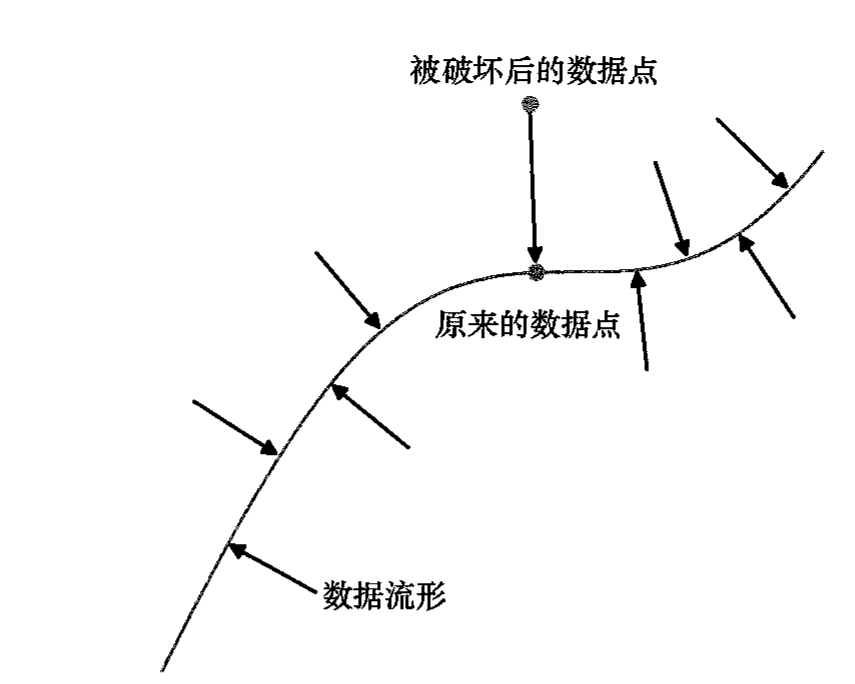
\includegraphics[width=0.52\textwidth]{ch19-fig513-denoise-manifold.png}
\caption{在去噪自编码器中，数据点被假定存在于数据空间中的一个低维流形上，并且被加性噪声破坏了。自编码器会学习将损坏的数据点映射回它们原来的值，因此自编码器为数据空间中的每个点学习了一个指向流形的向量}
\label{figure:ch19-去噪流形}
\end{figure}

\subsection{掩蔽自编码器}\label{subsection:ch19-掩蔽自编码器}

我们已经看到，借助随机遮盖输入子集的自监督学习方式，像 BERT 这样的 Transformer 模型能学习到自然语言的深层次内部表示（参见\cref{section:ch12-自然语言}）。人们很自然会问，类似的方法能应用于自然图像吗？

\begin{definition}[掩蔽自编码器]\label{definition:ch19-掩蔽自编码器}
\textbf{掩蔽自编码器}（masked autoencoder）（He，2021）利用深度神经网络，根据输入图像的损坏版本重建图像；这里的损坏（corruption）形式是掩蔽或删除输入图像的一部分。
\end{definition}

% SUPPLEMENT: parent=definition:ch19-掩蔽自编码器; kind=motivation; location=紧随其后的 remark（重构新增）
\begin{remark}（重构新增）
\cref{definition:ch19-掩蔽自编码器}是\cref{definition:ch19-去噪自编码器}的一个特例：损坏算子不再是加性噪声或随机置零，而是“删除一个补丁块”。这个特例之所以重要，是因为它把“去噪”与 Transformer 的 token 序列表示对接起来——被保留的补丁成为编码器的输入 token，被删除的补丁不再需要计算，于是编码器的计算量随掩蔽比例线性下降。这也解释了原书随后强调的“掩蔽的区块简单地被省略”与 BERT 用固定掩蔽符号替换的区别。

条件方面：损坏算子必须与后续任务无关（否则网络可以学会“猜出”掩蔽模式而不是图像结构）；掩蔽比例要足够高才能迫使网络学习全局结构，但过高会使可用信息不足；此外解码器必须能处理被恢复的完整 token 序列，这要求位置编码在掩蔽后仍能对齐原图网格。
\end{remark}

这种技术通常可以与视觉 Transformer 架构结合起来使用（参见\cref{subsection:ch12-视觉Transformer}），因为在这种情况下，仅仅通过传递随机选定的输入补丁标记（input patch token）子集给编码器，就可以轻松实现对输入图像的部分进行掩蔽。\cref{figure:ch19-掩蔽自编码器}总结了整个算法。

\begin{figure}[htbp]
\centering
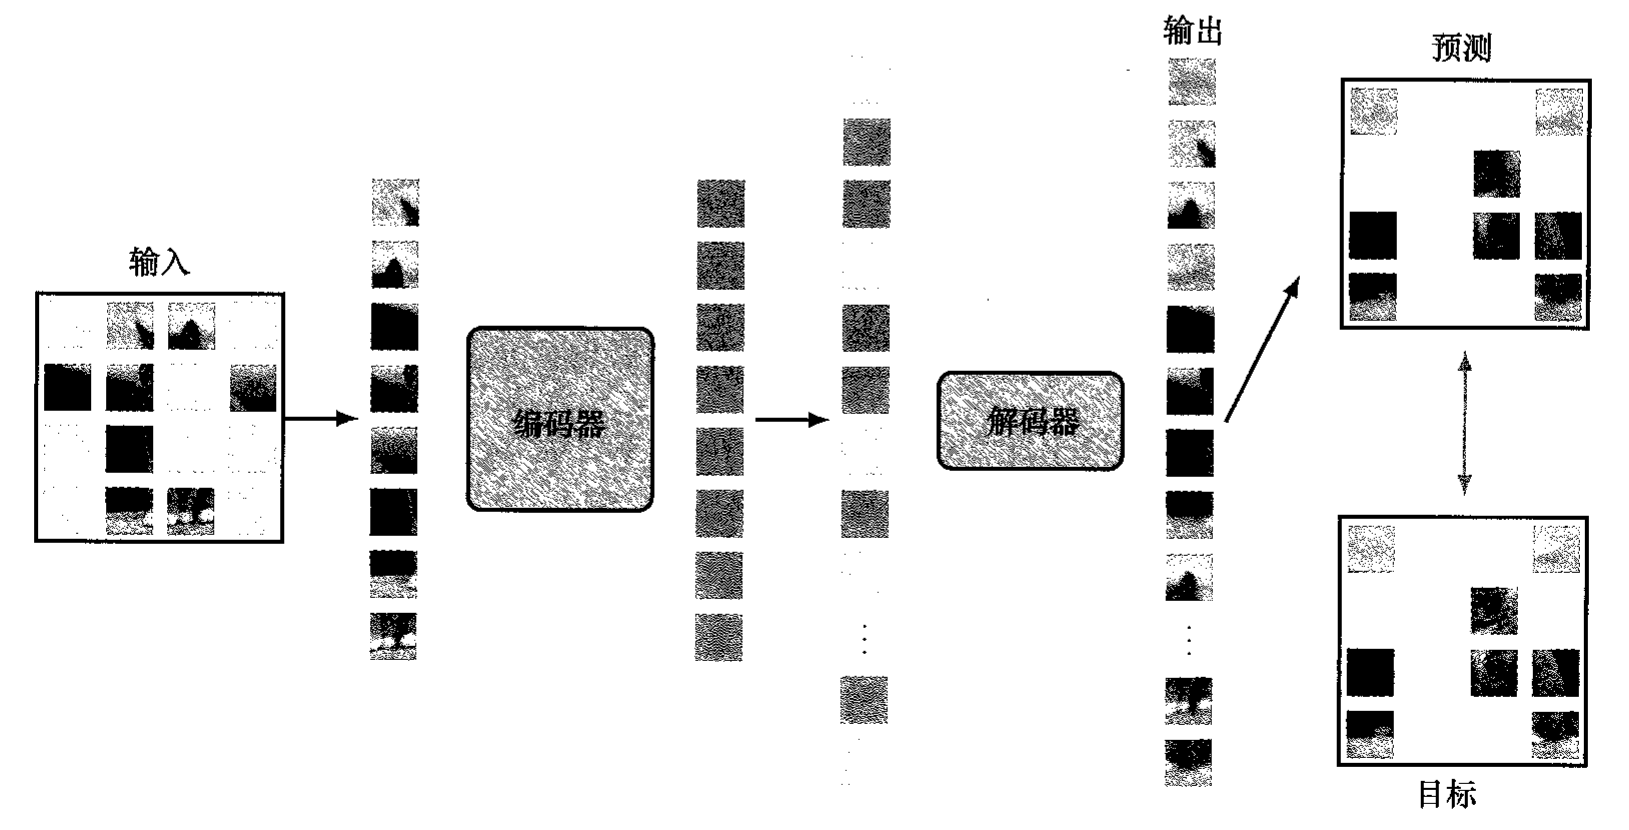
\includegraphics[width=0.88\textwidth]{ch19-fig513-mae.png}
\caption{掩蔽自编码器在训练阶段的架构。注意，目标是输入的补集，因为损失仅应用于被掩蔽的区块。训练结束后，解码器被丢弃，编码器用于将图像映射到内部表示，以便在后续任务中使用}
\label{figure:ch19-掩蔽自编码器}
\end{figure}

和语言不同，图像具有更多的冗余，并伴有强烈的局部相关性。在一句话中省略一个单词可能会大大增加歧义，然而随机移除图像中的一小块通常对图像的语义影响很小。当输入图像有较高掩蔽比例（通常为 $75\%$）时，算法能学到最佳的内部表示，而 BERT 中的掩蔽比例仅为 $15\%$。在 BERT 中，掩蔽的输入被固定的掩蔽符号替换；而在掩蔽自编码器中，掩蔽的区块简单地被省略。考虑到 Transformer 的计算效率随着输入序列长度的增加而下降，通过省略大量的输入区块，我们可以节省大量的计算资源，因此掩蔽自编码器成为预训练大型 Transformer 编码器的优选。

由于解码器层同样是 Transformer，它需要按照原始图像的维度来运作。因为 Transformer 的输出与输入具有相同的维度，我们需要在编码器输出和解码器输入之间恢复图像的维度。这可以通过重新引入被掩蔽的区块来实现，每个片段标记都增加了位置编码信息，并且由固定的掩蔽标记向量表示。由于解码器表示的维度远高于编码器，解码器 Transformer 拥有的可学习参数远少于编码器 Transformer。解码器的输出对接的是一个可学习的线性层，用于将输出表示映射到像素值空间，而训练损失函数的作用就是简单地对每个图像缺失区块的均方误差取平均值。

\begin{example}[ 掩蔽自编码器的图像重构]\label{example:ch19-掩蔽重构}
\cref{figure:ch19-掩蔽重构}展示了使用训练成功的掩蔽自编码器重建图像的 $4$ 个例子，展示了训练后的自编码器在生成合理语义上可信的重构能力。在每个例子中，被掩蔽的输入在左侧，重建的图像在中间，原始图像在右侧；被掩蔽的输入只剩少量可见补丁，而重建结果已经恢复了物体的整体轮廓与主要纹理。
\end{example}

\begin{figure}[htbp]
\centering
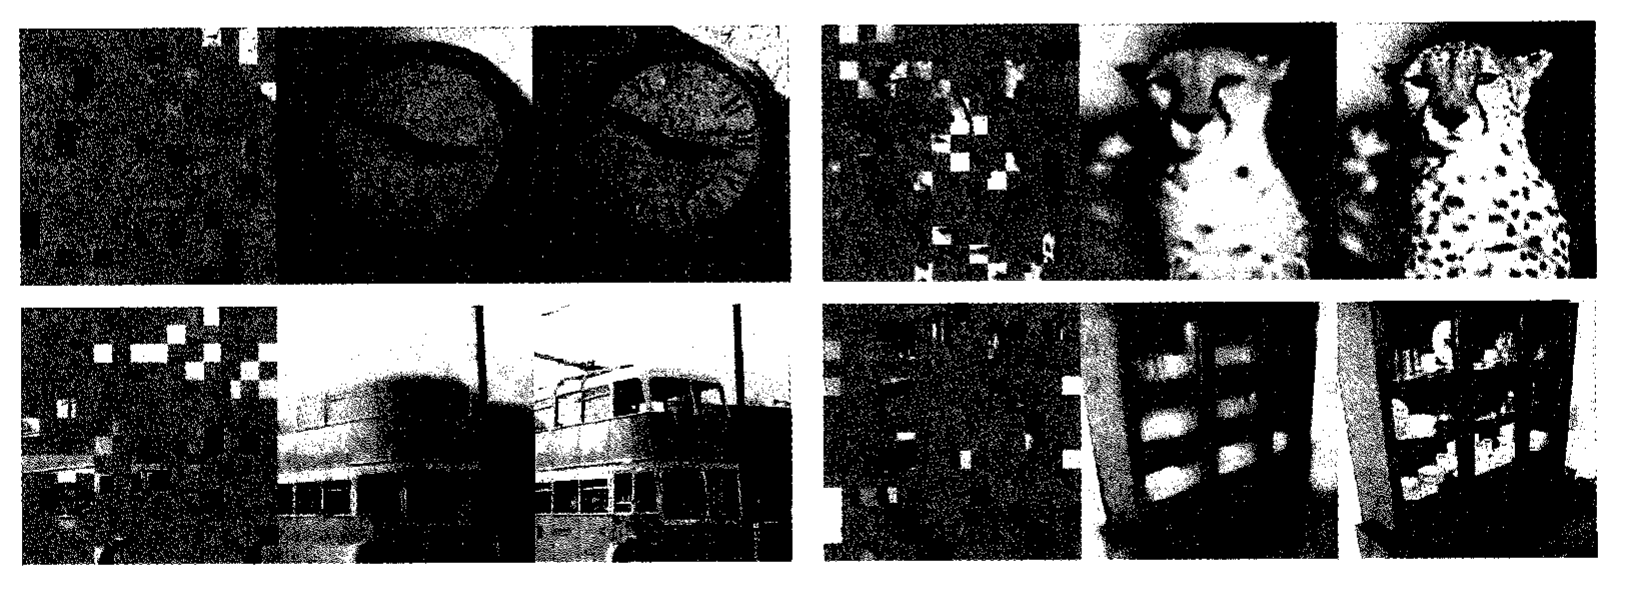
\includegraphics[width=0.86\textwidth]{ch19-fig514-mae-recon.png}
\caption{使用训练成功的掩蔽自编码器重建图像的 $4$ 个例子。在这些例子中，有 $80\%$ 的输入区块被掩蔽。在每个例子中，被掩蔽的图像在左侧，重建的图像在中间，原始图像在右侧 [图片来源于 He et al.(2021)，经授权使用]}
\label{figure:ch19-掩蔽重构}
\end{figure}

然而，我们最终的目标是学习对后续下游任务有用的内部表示，因此我们舍弃了解码器，而把编码器应用于没有遮蔽的完整图像，并配备了一组针对所需应用而微调的新输出层。请注意，虽然这一算法最初是为图像数据而设计的，但理论上可以应用于任何模态的数据。

\end{document}
